%%%%%%%%%%%%%%%%%%%%%%%%%%%%%%%%%%%%%%%%%
% Beamer Presentation
% LaTeX Template

\documentclass{beamer}
\mode<presentation> {
\usetheme{Warsaw}
}

\usepackage{multicol}
\usepackage[russian]{babel}
\usepackage{graphicx} 
\usepackage{hyperref}

\title[Introduction to Python]{Data structures \& Control Flow} 
\author{Sugarkhuu Radnaa} 
\institute[]
{
Py4Econ in Ulaanbaatar \\ 
\medskip
\textit{py4econ@gmail.com} 
}
\date{18 December, 2021}  % \today

\begin{document}

\begin{frame}
\titlepage % Print the title page as the first slide
\end{frame}

\begin{frame}
    \frametitle{Week 2: Learning objectives}
    Get to know: 
    \begin{enumerate}
        \item Basic data types in Python
        \item Data structures in \textbf{numpy} and \textbf{pandas}
        % \item Data file formats: \textbf{html, json, csv, pickle}
        \item \textbf{SQL} basics
        \item \textbf{if, else and elif} conditions
        \item \textbf{for and while} loop
    \end{enumerate}
\end{frame}

%------------------------------------------------
\section{Data types and structures} 
%------------------------------------------------

\begin{frame}
\frametitle{Data types in Python}
    \begin{enumerate}
        \item String
        \item Integer, Float, 
        \item Boolean
        \item Datetime
        \item List, tuple, set, dictionary
    \end{enumerate}
\end{frame}

\begin{frame}
    \frametitle{Operations on data}
        \begin{itemize}
            \item slice: d[1:10]
            \item update or add: d[a] = b
            \item remove or pop: d[a] = [] 
            \item join, concatenate: f = [d,e]
        \end{itemize}
\end{frame}

\begin{frame}
\frametitle{Main data structures in Python}
    \begin{itemize}
        \item Array (numpy)
        \item Dataframe (pandas)
    \end{itemize}
\end{frame}

\begin{frame}
    \frametitle{Numpy}
    Numpy and Scipy are extensively used for scientific computations and ML/AI algorithms
    \begin{itemize}
        \item random array and vector operations
        \item universal functions (sin, cos, max, argmax, ...)
        \item array handling (broadcast, tile, ravel, ...)
        \item matrix operations
    \end{itemize}
\end{frame}

% \begin{frame}
%     \frametitle{More on Numpy}
%     Powerful data manipulation package in Python
% \end{frame}

\begin{frame}
    \frametitle{Pandas}
    Powerful dataframe package in Python
        \begin{itemize}
            \item Can read data from many sources (csv, excel, json, html, url)
            \item Can handle large size of data
            \item Can sync well with other packages
        \end{itemize}
\end{frame}

\begin{frame}
    \frametitle{Operations in Pandas}
    \begin{enumerate}
        \item info, dtypes 
        \item head, tail 
        \item describe
        \item df[‘field’] = df.field
        \item loc, iloc
        \item sort, filter
        \item groupby, pivot table
        \item type conversion
        \item min, max, mean, sum
        \item import/export dataframe from/to file (csv, json, xlsx, ...)
    \end{enumerate}
\end{frame}

% \begin{Few words on files}
%     \frametitle{SQL}
%     \begin{enumerate}
%         \item head, tail
%         \item dtypes
%         \item describe
%         \item df[‘field’] = df.field
%         \item loc, iloc
%         \item sort, filter
%         \item groupby, pivot table
%         \item astype
%     \end{enumerate}
% \end{frame}

\begin{frame}
    \frametitle{SQL}
    SQL is the most popular database language. There are many different DBMS (database management system)s including SQL and NoSQL. \\
    \textbf{Popular SQL databases}:
    \begin{enumerate}
        \item Oracle SQL
        \item Microsoft SQL
        \item MySQL
        \item PostgreSQL
    \end{enumerate}    

    \textbf{Popular NoSQL databases}:
    \begin{enumerate}
        \item MongoDB
        \item ElasticSearch
        \item Casandra
    \end{enumerate}    
\end{frame}

\begin{frame}
    \centering
    \frametitle{Sample database (SQL) design}
    \begin{flushleft}
        Data architecture is a crucial in any organization. When due implemented, it can become a game changing factor. Efficient ETL, Datawarehouse and 
        data centers are necessary for an efficient DBMS.        
    \end{flushleft}
    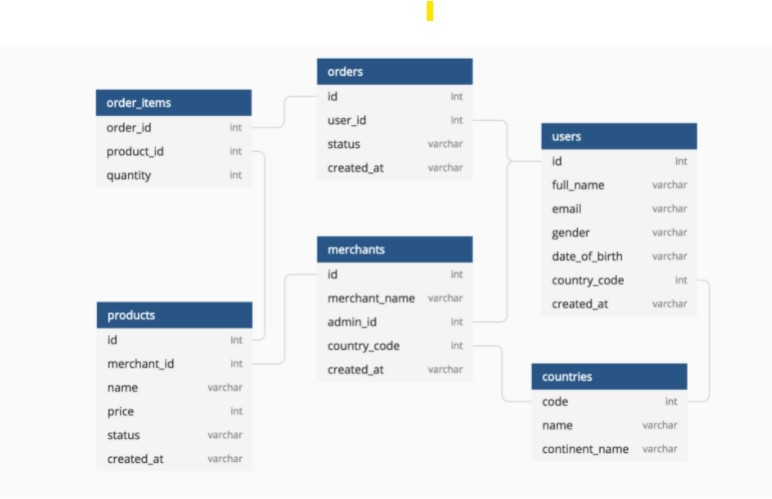
\includegraphics[scale=0.5]{figures/db_design.jpg}
\end{frame}

\begin{frame}
    \frametitle{SQL: W3SCHOOL examples}
    \begin{enumerate}
\tiny        \item SELECT CustomerName, City FROM Customers; 
        \item SELECT * FROM Customers
        WHERE Country='Mexico';
        \item SELECT * FROM Customers
        WHERE Country='Germany' AND (City='Berlin' OR City='München');
        \item UPDATE Customers
        SET ContactName = 'Alfred Schmidt', City= 'Frankfurt'
        WHERE CustomerID = 1;
        \item SELECT * FROM Customers
        WHERE ContactName LIKE 'a%o';
        \item SELECT Customers.CustomerName, Orders.OrderID
        FROM Customers
        LEFT JOIN Orders ON Customers.CustomerID = Orders.CustomerID
        ORDER BY Customers.CustomerName;
        \item SELECT COUNT(CustomerID), Country
        FROM Customers
        GROUP BY Country
        ORDER BY COUNT(CustomerID) DESC;
    \end{enumerate}
\end{frame}


%------------------------------------------------
\section{Control Flow} 
%------------------------------------------------

\begin{frame}
    \frametitle{Contiditional statements}
    \begin{itemize}
        \item if statement:
        \item else:
        \item elif (else if) statement:  
        \item and, or, in, isinstance
    \end{itemize}
\end{frame}

\begin{frame}
    \frametitle{Loops (repeat an action)}
    \begin{itemize}
        \item For - used only when we already knew the number of iterations
        \item While - used only when the number of iteration are not exactly known
    \end{itemize}

    Ways to exit loop:
    \begin{itemize}
        \item break
        \item continue
    \end{itemize}
    
    Use 'pass' when operation within the loop is not implemented yet
\end{frame}

%------------------------------------------------
\section{Homework} 
%------------------------------------------------

\begin{frame}
    \frametitle{Homework}
    \begin{enumerate}
        \item Task 1
        \item Task 2
        \item Task 3
    \end{enumerate}

    \vskip 2mm
    \begin{itemize}
        \item Submit your result as a Github repository
        \item Deadline: 15 January, 2022
    \end{itemize}

\vfill
\textbf{Note:} Create a github repo from the start and populate it with your results step by step.
\end{frame}

\begin{frame}
    \frametitle{Task 1}
    \begin{enumerate}
        \item Add rows with arbitrary values to “data.xlsx” so that you have 50 rows in total
        \item Create a '.csv' file with data of only women older than 25 years old
            \begin{enumerate}
                \item filter by using only loops
                \item filter by using conditions in pandas 
            \end{enumerate}
        \item Create a '.json' file with data of men under than 23 years old
            \begin{enumerate}
                \item filter by using only loops
                \item filter by using conditions in pandas 
            \end{enumerate}
    \end{enumerate}
\end{frame}

\begin{frame}
    \frametitle{Task 2}
    \begin{enumerate}
        \item What are the values in row 17 and column 2-5 of dataframe created from "data.xlsx"
        \item What are the values row 25-28 and column 'firstName, age' of dataframe created from "data.xlsx"
        \item Find the lowest, the highest and mean salary and age for men and women separately using 'groupby'
        \item Find the lowest, the highest and mean salary and age for men and women separately using 'pivot table'
    \end{enumerate}
\end{frame}

% \begin{frame}
%     \frametitle{Task 3: Numpy}
%     \begin{enumerate}
%         \item What are the values in row 17 and column 2-5 of dataframe created from "data.xlsx"
%         \item What are the values row 25-28 and column 'firstName, age' of dataframe created from "data.xlsx"
%         \item Find the lowest, the highest and mean salary and age for men and women separately using 'groupby'
%         \item Find the lowest, the highest and mean salary and age for men and women separately using 'pivot table'
%     \end{enumerate}
% \end{frame}

\begin{frame}
    \frametitle{Task 3}
    \begin{enumerate}
        \item Populate a MySQL (or PostgreSQL) table by the data in “data.xlsx” (CREATE TABLE)
        \item Select 'firstName' and 'lastName' of the first three rows  ('LIMIT')
        \item Select 'firstName' and 'age' of the last three rows ('ORDER BY, LIMIT')
    \end{enumerate}
\vfill
\textbf{Tip:} Watch the following tutorial for MySQL (PostgreSQL)
\begin{itemize}
    \item \href{https://www.youtube.com/watch?v=e1LPfehYSgg&list=PLS1QulWo1RIY4auvfxAHS9m_fZJ2wxSse}{MySQL}
    \item \href{https://www.youtube.com/watch?v=xaWlS9HtWYw}{PostgreSQL}
\end{itemize}
\end{frame}

\begin{frame}
\Huge{\centerline{Thank you!}}
\end{frame}

%----------------------------------------------------------------------------------------

\end{document} 